\section{Layers}
\subsection{Physical}
  \begin{frame}
    \frametitle{Aims}
      \begin{itemize}
        \item Interface data link layer,\pause
        \item (De)Encode,\pause
        \item Transmit: 1 after 0 (after 0 or 1, after 0... or 1)
      \end{itemize}
  \end{frame}
  \begin{frame}
    \frametitle{Hardware medium}
      \begin{itemize}
        \item IEEE 802.3 (a.k.a. Ethernet): $<$100Gbit/s \pause
        \item IEEE 802.11 (a.k.a. Wi-Fi): $<$50 Mbit/s (802.11ad goes up to 6.75 Gbit/s) \pause
        \item IEEE 802.15.1 (a.k.a. Bluetooth): $<$1 Mbit/s \pause
        \item IEEE 802.15.4 (a.k.a. ZigBee): $<$250 kbit/s \pause
        \item IEEE 802.16 (a.k.a. Wi-Max): $<$40 Mbit/s \pause
        \item IEEE 1394 (a.k.a. Firewire): $<$3200 Mbit/s \pause
        \item USB, serial port such as RS-232...
      \end{itemize}
  \end{frame}
  \begin{frame}
    \frametitle{Hardware medium: IEEE 802.3 (Ethernet)}
    \begin{figure}[t]
      \centering
      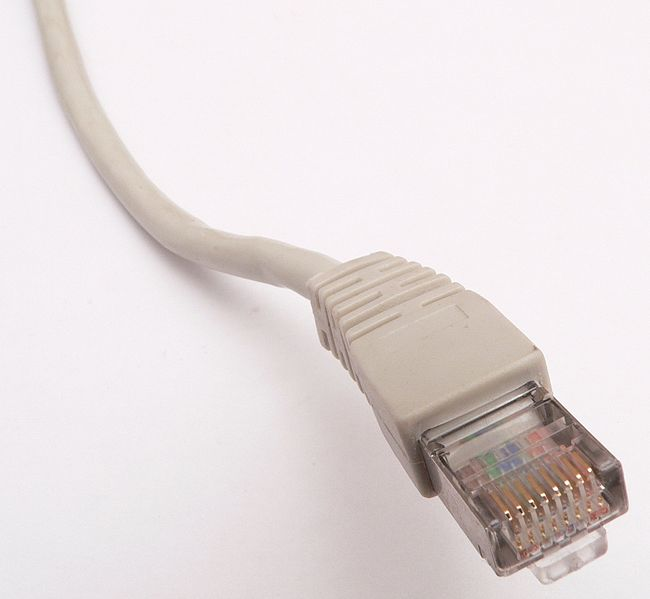
\includegraphics[height=5cm]{./imgs/rj45.jpg}
      \caption{\color{blue}\href{https://en.wikipedia.org/wiki/File:Ethernet_RJ45_connector_p1160054.jpg}{RJ45 connector}}
      \label{fig:rj45}
    \end{figure}
  \end{frame}
  \begin{frame}
    \frametitle{Hardware medium: IEEE 802.15.1 (Bluetooth)}
    \begin{figure}[t]
      \centering
      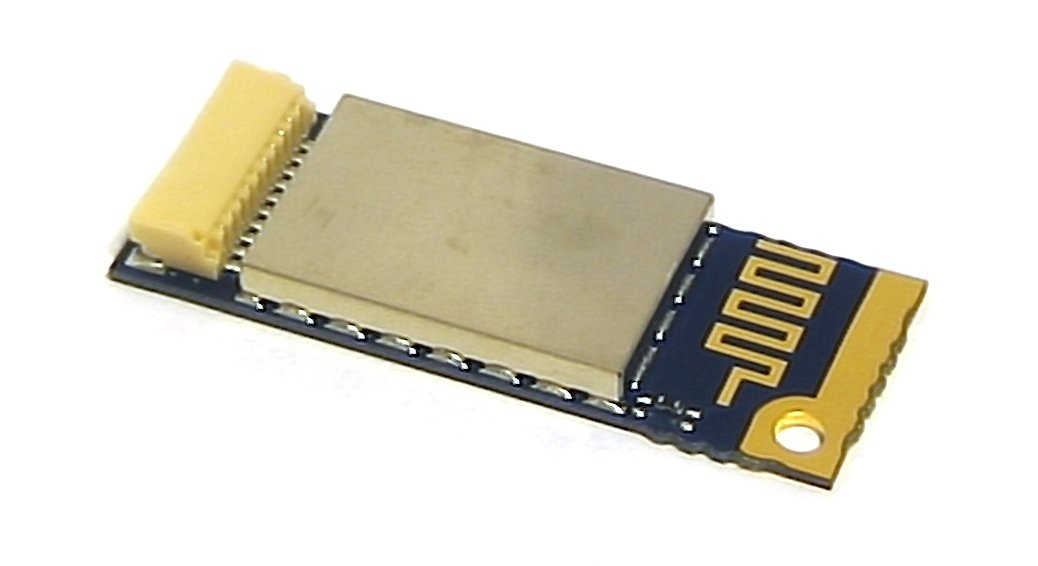
\includegraphics[height=5cm]{./imgs/bluetooth_card}
      \caption{\color{blue}\href{https://upload.wikimedia.org/wikipedia/commons/2/28/DELL_TrueMobile_350_Bluetooth_card.jpg}{Bluetooth card}}
      \label{fig:bluetooth_card}
    \end{figure}
  \end{frame}
  \begin{frame}
    \frametitle{Hardware medium: IEEE 802.15.4 (ZigBee)}
    \begin{figure}[t]
      \centering
      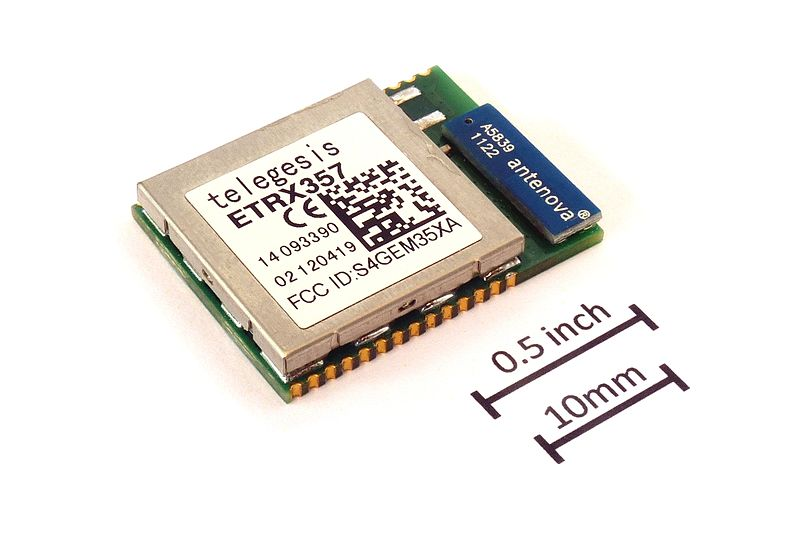
\includegraphics[height=5cm]{./imgs/zigbee.jpg}
      \caption{\color{blue}\href{https://upload.wikimedia.org/wikipedia/commons/thumb/2/29/ETRX357_ZigBee_module_with_size_ref.JPG/800px-ETRX357_ZigBee_module_with_size_ref.JPG}{ZigBee card}}
      \label{fig:ZigBee}
    \end{figure}
  \end{frame}
  \begin{frame}
    \frametitle{Hardware medium: IEEE 802.16 (Wi-Max)}
    \begin{figure}[t]
      \centering
      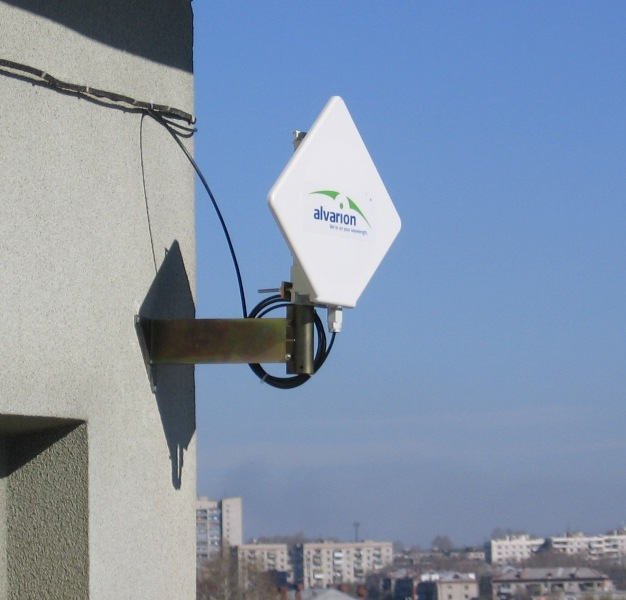
\includegraphics[height=5cm]{./imgs/Wi-Max.jpg}
      \caption{\color{blue}\href{https://upload.wikimedia.org/wikipedia/commons/d/db/Alvarion_CPE.jpg}{Wi-Max antenna}}
      \label{fig:Wi-Max_antenna}
    \end{figure}
  \end{frame}
  \begin{frame}
    \frametitle{Hardware medium: IEEE 1394 (Firewire)}
    \begin{figure}[t]
      \centering
      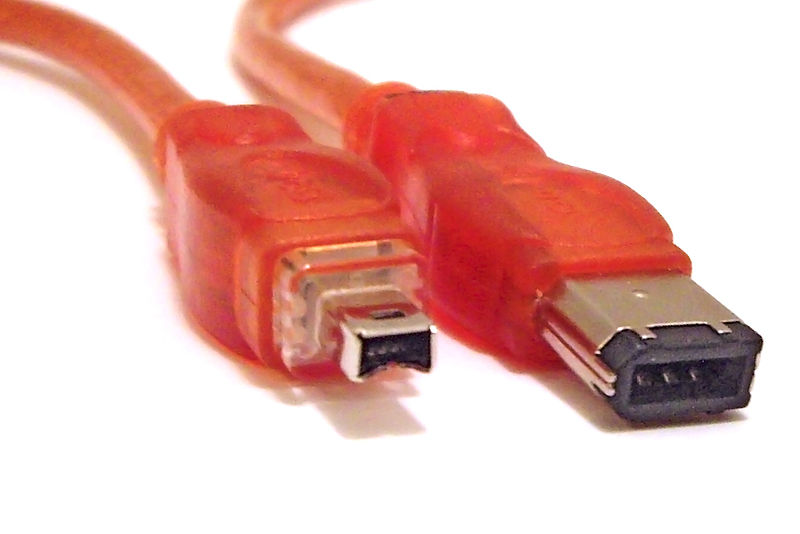
\includegraphics[height=5cm]{./imgs/firewire.jpg}
      \caption{\color{blue}\href{https://upload.wikimedia.org/wikipedia/commons/thumb/f/f7/FireWire_cables.jpg/800px-FireWire_cables.jpg}{Firewire connector}}
      \label{fig:firewire}
    \end{figure}
  \end{frame}
  \begin{frame}
    \frametitle{Encoding}
      \begin{itemize}
        \item \textbf{MLT3 (Multi-Level Transmit):} state change for 1s over 3 levels, stay in the same state for 0s \pause
        \item \textbf{AMI (Alternate Mark Inversion):} state 0 for 0s, state +/-1 for 1s \pause
        \item \textbf{Manchester:} voltage transition (rising/falling edge mean 1/0) \pause
        \item \textbf{BMC (Biphase Mark Code):} change its state for 1s, stay on the same state for 0s \pause
        \item and so on...
      \end{itemize}
  \end{frame}
  \begin{frame}
    \frametitle{Encoding: Multi-Level Transmit}
    \begin{figure}[t]
      \centering
      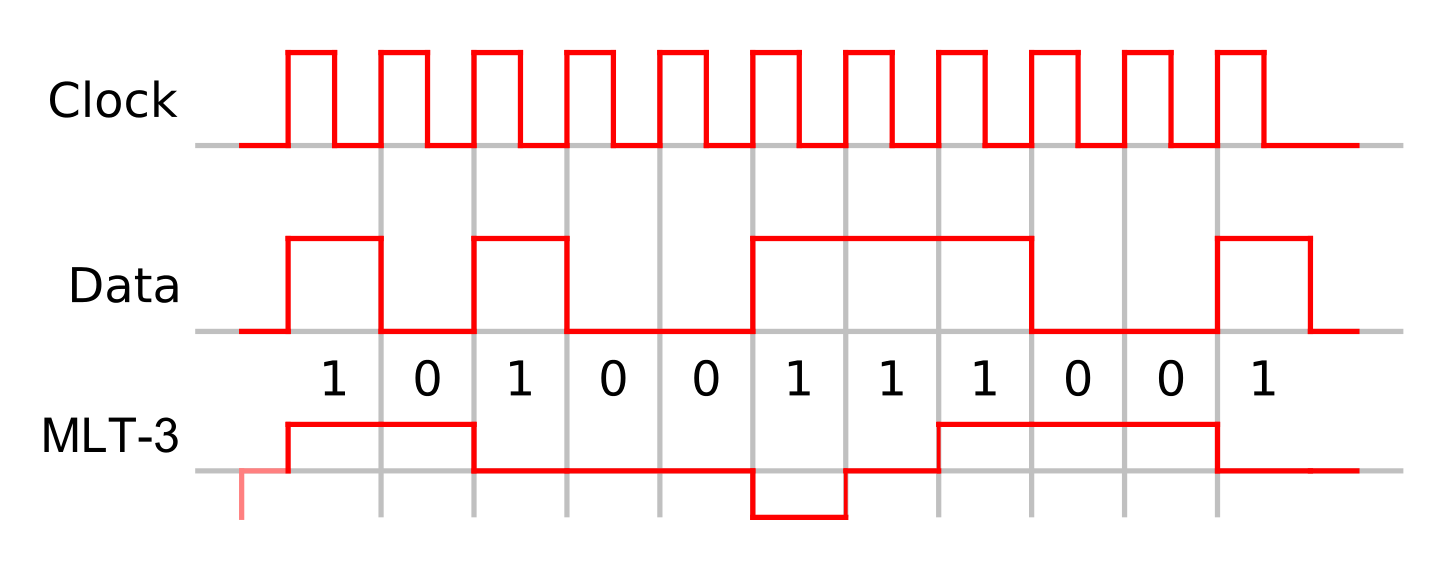
\includegraphics[height=3cm]{./imgs/mlt3.png}
      \caption{\color{blue}\href{https://upload.wikimedia.org/wikipedia/commons/thumb/b/b4/MLT3encoding.svg/1456px-MLT3encoding.svg.png}{Multi-Level Transmit}}
      \label{fig:mlt3}
    \end{figure}
  \end{frame}
  \begin{frame}
    \frametitle{Encoding: Alternate Mark Inversion}
    \begin{figure}[t]
      \centering
      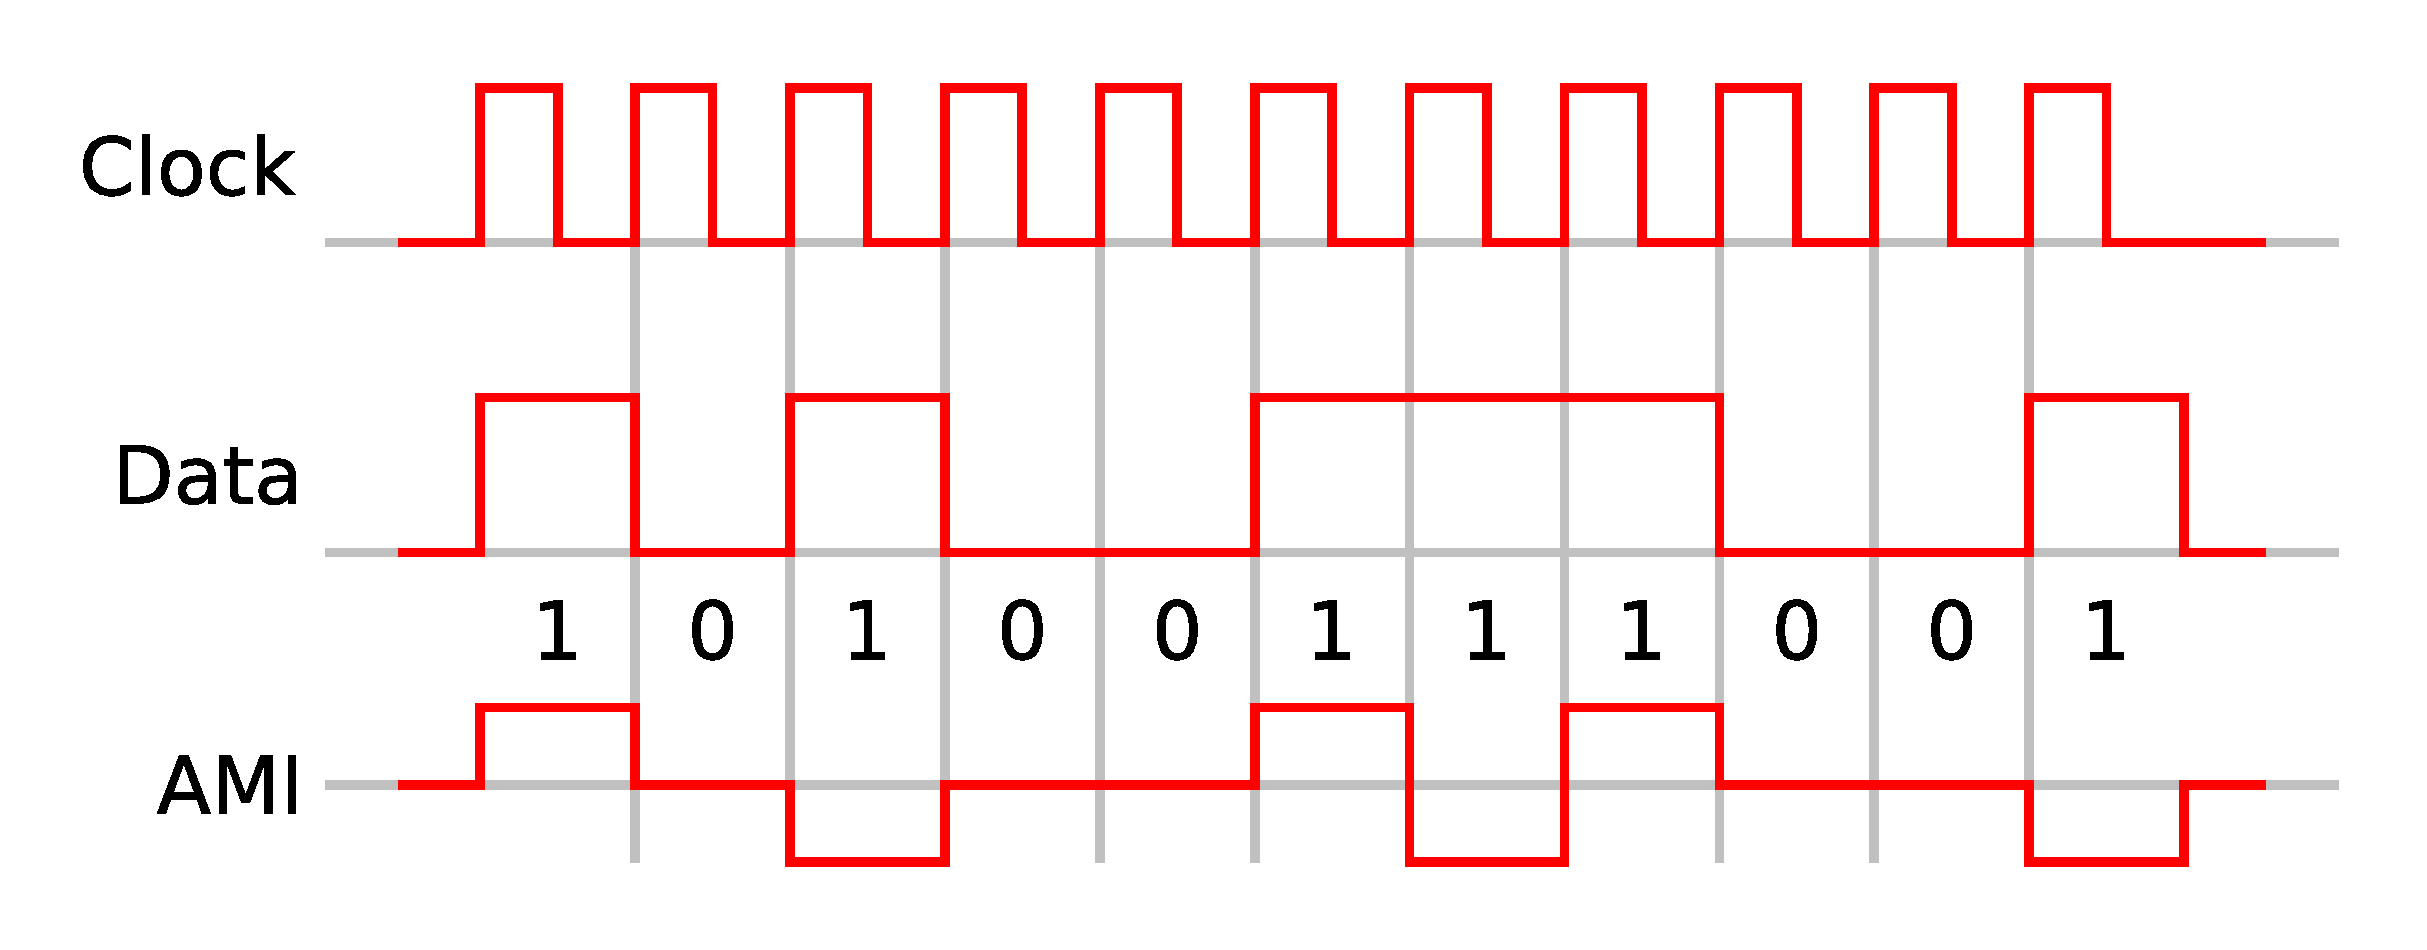
\includegraphics[height=3cm]{./imgs/ami.pdf}
      \caption{\color{blue}\href{https://upload.wikimedia.org/wikipedia/commons/b/b6/Ami_encoding.svg}{Alternate Mark Inversion}}
      \label{fig:ami}
    \end{figure}
  \end{frame}
  \begin{frame}
    \frametitle{Encoding: Manchester}
    \begin{figure}[t]
      \centering
      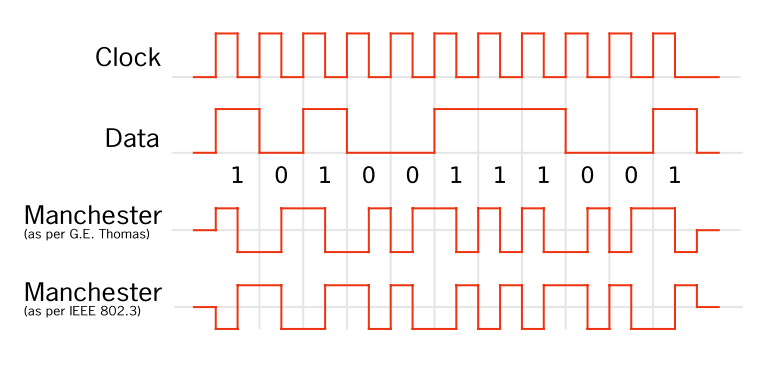
\includegraphics[height=3cm]{./imgs/manchester.png}
      \caption{\color{blue}\href{https://upload.wikimedia.org/wikipedia/commons/thumb/9/90/Manchester_encoding_both_conventions.svg/771px-Manchester_encoding_both_conventions.svg.png}{Manchester}}
      \label{fig:manchester}
    \end{figure}
  \end{frame}
  \begin{frame}
    \frametitle{Encoding: Biphase Mark Code}
    \begin{figure}[t]
      \centering
      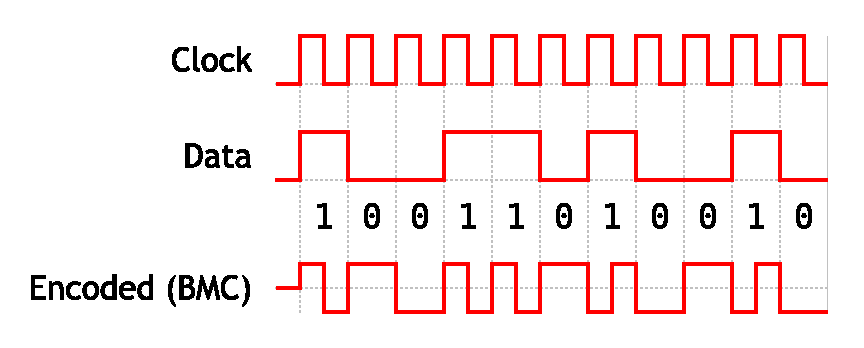
\includegraphics[height=3cm]{./imgs/bmc.pdf}
      \caption{\color{blue}\href{https://upload.wikimedia.org/wikipedia/commons/c/cb/Biphase_Mark_Code.svg}{Biphase Mark Code}}
      \label{fig:bmc}
    \end{figure}
  \end{frame}
  \begin{frame}
    \frametitle{Transmitting}
    \begin{figure}[t]
      \centering
      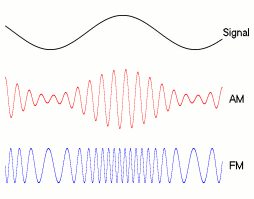
\includegraphics[height=5cm]{./imgs/modulation.png}
      \caption{\color{blue}\href{https://upload.wikimedia.org/wikipedia/commons/a/a4/Amfm3-en-de.gif}{Amplitude and phase modulation}}
      \label{fig:modulation}
    \end{figure}
  \end{frame}
  \begin{frame}
    \frametitle{Error detection}
      \begin{itemize}
        \item Repetition (hum...) \pause
        \item Parity (XOR) \pause
        \item Checksum \pause
        \item CRC (Cyclic redundancy check): with a polynomial divison \pause
        \item Hash \pause
        \item and so on...
      \end{itemize}
  \end{frame}
  \begin{frame}
    \frametitle{Error correcting}
      \begin{itemize}
        \item Repetition (again) \pause
        \item Hamming \pause
        \item MDPC (Multidimensional parity-check code)
      \end{itemize}
  \end{frame}

  \begin{frame}
    \frametitle{Correction: MDPC}
    Raw data to send: 0x01 02 03 04
      \begin{figure}[h]
      \centering
      \begin{tabular}{cc|c}
        0x01 & 0x02 & 0x03 \\
        0x03 & 0x04 & 0x07 \\ \hline
        0x04 & 0x06 &
      \end{tabular}
      \caption{Data received with MDPC}
      \label{fig:ami}
    \end{figure}
  Data sent (with MDPC): 0x01 02 03 03 04 07 04 06
  \end{frame}
\subsection{Data Link}
  \begin{frame}
    \frametitle{Aims}
      \begin{itemize}
        \item Interface network layer,\pause
        \item Delivery to unique(?) hardware addresses,\pause
        \item Framing,\pause
        \item Data transfer
      \end{itemize}
  \end{frame}
  \begin{frame}
    \frametitle{Layer composition (of its two sublayers)}
      \begin{enumerate}
        \item Logical Link Control (LLC):
          \begin{itemize}
            \item end to end flow control
            \item end to end error control
            \item (transmitting/receiving) protocols, over MAC sublayer, multiplexing
          \end{itemize}\pause
        \item Media Access Control (MAC):
          \begin{itemize}
            \item physical (hardware) addressing
            \item collision detection and retransmission
            \item data packet scheduling (and queuing)
            \item QoS
            \item VLAN
          \end{itemize}
      \end{enumerate}
  \end{frame}
  \begin{frame}
    \frametitle{Carrier Sense Multiple Access with Collision Avoidance}
    \begin{figure}[t]
      \centering
      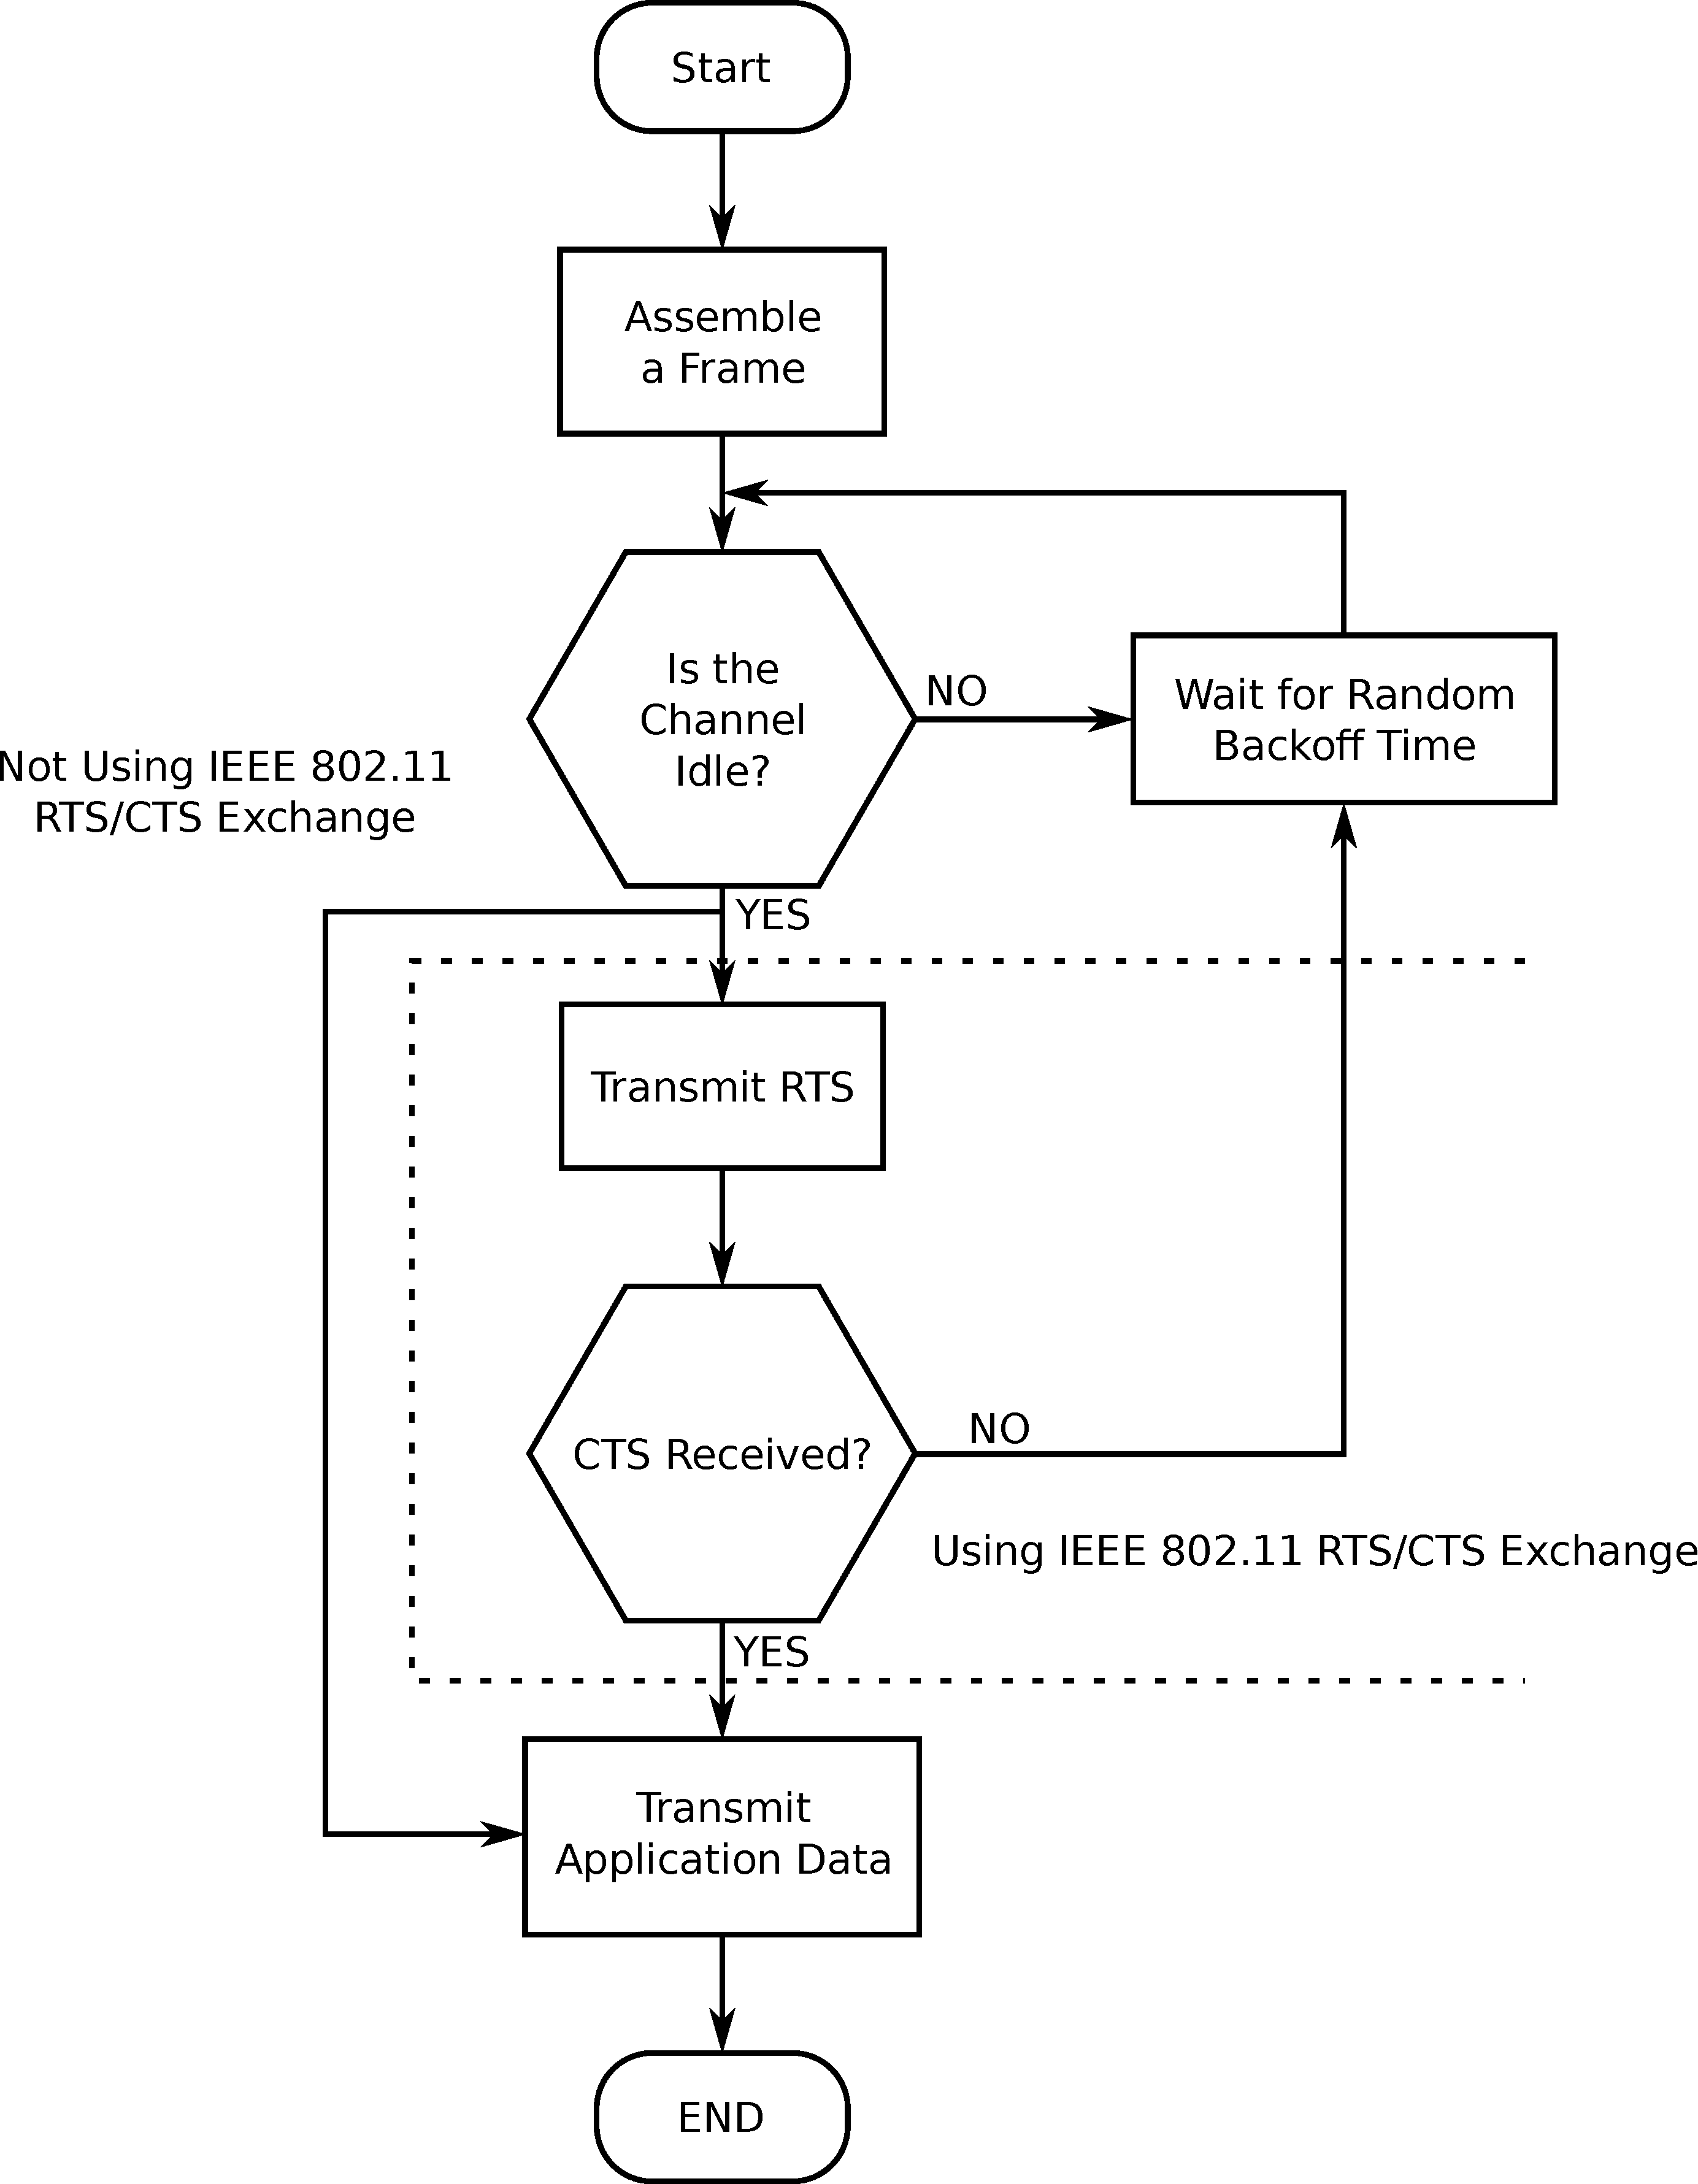
\includegraphics[height=6cm]{./imgs/csma_ca.pdf}
      \caption{\color{blue}\href{https://en.wikipedia.org/wiki/File:Csma_ca.svg}{CSMA CA}}
      \label{fig:csma_ca}
    \end{figure}
    \end{frame}
  \begin{frame}
    \frametitle{Layer 2 Ethernet packet}
      \begin{figure}[h]
      \centering
      \begin{tabular}{|c|c|c|c|c|c|c|c|c|}
        \hline
        \multicolumn{3}{|c|}{MAC dest. (\color{blue}6\color{black})} & \multicolumn{3}{|c|}{MAC src. (\color{blue}6\color{black})} & \multicolumn{2}{|c|}{\color{brown}VLAN tag* (\color{blue}4\color{brown})\color{black}} & Ethertype (\color{blue}2\color{black}) \\ \hline
        \multicolumn{6}{|c|}{Payload (\color{blue}42-1500\color{black})} & \multicolumn{3}{|c|}{Frame check sequence (\color{blue}4\color{black})}\\ \hline
      \end{tabular}
      \caption{Layer 2 Ethernet packet}
      \label{fig:eth_packet}
    \end{figure}
    \hfill \color{brown}optional\color{black}, Content (\color{blue}size in bytes\color{black})
    \begin{figure}[h]
      \centering
      \begin{tabular}{|c|c|}
        \hline
        \textbf{Ethertype 0x} & \textbf{Protocol} \\ \hline
        0800 & IPv4 \\ \hline
        0806 & ARP \\ \hline
        0842 & Wake-on-LAN \\ \hline
        86dd & IPv6 \\ \hline
      \end{tabular}
      \caption{Data received with MDPC}
      \label{fig:eth_type}
    \end{figure}
  \end{frame}


  \begin{frame}
    \frametitle{ARP example}
      \begin{figure}
      \centering
      \resizebox{11.5cm}{!} {
        \begin{tabular}{lcccccccccccccccc}
          \textbf{0000} & ff & ff & ff & ff & ff & ff & fa & ba & 00 & ab & ab & af & 08 & 06 & 00 & 01 \\
          \textbf{0010} & 08 & 00 & 06 & 04 & 00 & 01 & fa & ba & 00 & ab & ab & af & ac & 11 & 22 & 37 \\
          \textbf{0020} & 00 & 00 & 00 & 00 & 00 & 00 & ac & 11 & 00 & f9 & 00 & 00 & 00 & 00 & 00 & 00 \\
          \textbf{0030} & 00 & 00 & 00 & 00 & 00 & 00 & 00 & 00 & 00 & 00 & 00 & 00 \\
        \end{tabular}
      }
      \caption{ARP request}
      \label{fig:arp_packet_ex}
    \end{figure}
        MAC address destination MAC address source Ethertype Hardware type Protocol type OpCode (1 request, 2 reply) IP address source IP address destination
  \end{frame}

  \begin{frame}
    \frametitle{ARP example}
      \begin{figure}
      \centering
      \resizebox{11.5cm}{!} {
        \begin{tabular}{lcccccccccccccccc}
          \textbf{0000} & \color{red}ff & \color{red}ff & \color{red}ff & \color{red}ff & \color{red}ff & \color{red}ff & \color{Marroon}fa & \color{Marroon}ba & \color{Marroon}00 & \color{Marroon}ab & \color{Marroon}ab & \color{Marroon}af & \color{blue}08 & \color{blue}06 & \color{magenta}00 & \color{magenta}01 \\
          \textbf{0010} & \color{OliveGreen}08 & \color{OliveGreen}00 & \color{gray}06 & \color{gray}04 & \color{fuchsia}00 & \color{fuchsia}01 & \color{Marroon}fa & \color{Marroon}ba & \color{Marroon}00 & \color{Marroon}ab & \color{Marroon}ab & \color{Marroon}af & \color{brown}ac & \color{brown}11 & \color{brown}22 & \color{brown}37 \\
          \textbf{0020} & \color{red}00 & \color{red}00 & \color{red}00 & \color{red}00 & \color{red}00 & \color{red}00 & \color{orange}ac & \color{orange}11 & \color{orange}00 & \color{orange}f9 & 00 & 00 & 00 & 00 & 00 & 00 \\
          \textbf{0030} & 00 & 00 & 00 & 00 & 00 & 00 & 00 & 00 & 00 & 00 & 00 & 00 \\
        \end{tabular}
      }
      \caption{ARP request}
      \label{fig:arp_req_ex-colored}
    \end{figure}
    \color{red}MAC address destination \color{Marroon}MAC address source \color{blue}Ethertype \color{magenta}Hardware type \color{OliveGreen}Protocol type \color{fuchsia}OpCode (1 request, 2 reply) \color{brown} IP address source \color{orange} IP address destination
  \end{frame}
  \begin{frame}
    \frametitle{ARP example}
      \begin{figure}
      \centering
      \resizebox{11.5cm}{!} {
        \begin{tabular}{lcccccccccccccccc}
          \textbf{0000} & fa & ba & 00 & ab & ab & af & be & be & 00 & 00 & eb & eb & 08 & 06 & 00 & 01 \\
          \textbf{0010} & 08 & 00 & 06 & 04 & 00 & 01 & be & be & 00 & 00 & eb & eb & ac & 11 & 00 & f9 \\
          \textbf{0020} & fa & ba & 00 & ab & ab & af & ac & 11 & 22 & 37 & 00 & 00 & 00 & 00 & 00 & 00 \\
          \textbf{0030} & 00 & 00 & 00 & 00 & 00 & 00 & 00 & 00 & 00 & 00 & 00 & 00 \\
        \end{tabular}
      }
      \caption{ARP reply}
      \label{fig:arp_rep_ex}
    \end{figure}
        MAC address destination MAC address source Ethertype Hardware type Protocol type OpCode (1 request, 2 reply) IP address source IP address destination
  \end{frame}
  \begin{frame}
    \frametitle{ARP example}
      \begin{figure}
      \centering
      \resizebox{11.5cm}{!} {
        \begin{tabular}{lcccccccccccccccc}
          \textbf{0000} & \color{red}fa & \color{red}ba & \color{red}00 & \color{red}ab & \color{red}ab & \color{red}af & \color{Marroon}be & \color{Marroon}be & \color{Marroon}00 & \color{Marroon}00 & \color{Marroon}eb & \color{Marroon}eb & \color{blue}08 & \color{blue}06 & \color{magenta}00 & \color{magenta}01 \\
          \textbf{0010} & \color{OliveGreen}08 & \color{OliveGreen}00 & \color{gray}06 & \color{gray}04 & \color{fuchsia}00 & \color{fuchsia}01 & \color{Marroon}be & \color{Marroon}be & \color{Marroon}00 & \color{Marroon}00 & \color{Marroon}eb & \color{Marroon}eb & \color{brown}ac & \color{brown}11 & \color{brown}00 & \color{brown}f9 \\
          \textbf{0020} & \color{red}fa & \color{red}ba & \color{red}00 & \color{red}ab & \color{red}ab & \color{red}af & \color{orange}ac & \color{orange}11 & \color{orange}22 & \color{orange}37 & 00 & 00 & 00 & 00 & 00 & 00 \\
          \textbf{0030} & 00 & 00 & 00 & 00 & 00 & 00 & 00 & 00 & 00 & 00 & 00 & 00 \\
        \end{tabular}
      }
      \caption{ARP reply}
      \label{fig:arp_rep_ex-colored}
    \end{figure}
    \color{red}MAC address destination \color{Marroon}MAC address source \color{blue}Ethertype \color{magenta}Hardware type \color{OliveGreen}Protocol type \color{fuchsia}OpCode (1 request, 2 reply) \color{brown} IP address source \color{orange} IP address destination
  \end{frame}

  \subsection{Network}
  \begin{frame}
    \frametitle{Aims}
      \begin{itemize}
        \item Interface transport layer,\pause
	\item Host addressing,\pause
        \item End-to-end packet transmission (data link? Connectionless? Switch? Router?),\pause
        \item Routing, load balancing
      \end{itemize}
  \end{frame}
  \subsubsection{IP addressing}
  \begin{frame}
    \frametitle{Concepts}
      \begin{itemize}
        \item IP addressing fundamentals,\pause
        \item Classfull IP addressing,\pause
        \item Subnet masks,\pause
        \item Variable length subnet masks (VLSM),\pause
        \item Classless inter-domain routing (CIDR).
      \end{itemize}
  \end{frame}

  \begin{frame}
    \frametitle{IP addressing fundamentals}
    \begin{block}{IP address}
      \begin{figure}
        \centering
        \begin{tabular}{|c|c|}
          \multicolumn{2}{c}{32 bits (4x4 bytes)} \\ \hline
           \multicolumn{2}{|c|}{\color{brown}mask} \\ \hline
          \color{brown}Networks part & \color{blue}Host part \\ \hline
        \end{tabular}
        \caption{IP address parts}
        \label{fig:inside_ip_address}
      \end{figure}
    \end{block}
  \end{frame}

  \begin{frame}
    \frametitle{IP addressing fundamentals}
    \begin{block}{Masks}
      \begin{itemize}
        \item Separates network and host bits,\pause
        \item MSB \textbf{always} are ones and then zeros! 255.254.255.0 is not possible,\pause
        \item Indicates how many bits are used for the network part:
        \begin{itemize}
          \item A 8-bit mask leaves 24 bits for the hosts,
          \item A 16-bit mask leaves 16 bits for the hosts,
          \item A 24-bit mask leaves 8 bits for the hosts,
          \item A N-bit mask leaves 32-N bits for the hosts.
        \end{itemize}\pause
        \item Two different mask (differences seen further):
        \begin{itemize}
          \item Network mask,
          \item Subnet mask.
        \end{itemize}
      \end{itemize}
    \end{block}
  \end{frame}
  \begin{frame}
    \frametitle{IP addressing fundamentals}
    \begin{block}{IP address}
      \begin{figure}
        \centering
        \begin{tabular}{|c|c|}
          \multicolumn{2}{c}{32 bits (4x4 bytes)} \\ \hline
          \uncover<2->{\color{brown}ones mask} & \uncover<2->{\color{blue}zeros mask} \\ \hline
          \color{brown}Networks part & \color{blue}Host part \\ \hline
        \end{tabular}
        \caption{IP address parts and mask}
        \label{fig:inside_ip_address_mask}
      \end{figure}
    \end{block}
  \end{frame}

  \begin{frame}
    \frametitle{IP addressing fundamentals}
    \begin{block}{Is that a host?}
      \begin{itemize}
        \item Network address,\pause
        \item Nodes,\pause
        \item Broadcast address.\pause
      \end{itemize}
    \end{block}
    \begin{block}{Within the same network}
      \begin{itemize}
        \item All addresses have the same network bits,\pause
        \item All nodes have different host bits,\pause
        \item Network address has zeros for host bits,\pause
        \item Broadcast address has ones for host bits.
      \end{itemize}
    \end{block}
  \end{frame}

  \begin{frame}
    \frametitle{Example: network 1}
    \begin{figure}
        \centering
      \begin{tabular}{|r|cccc|}
        \hline
        \multirow{2}{*}{Mask /24} & {\color{brown}255} & {\color{brown}255} & {\color{brown}255} & {\color{brown}0} \\
        & {\color{brown}11111111} & {\color{brown}11111111} & {\color{brown}11111111} & {\color{brown}00000000} \\ \hline
        \multirow{2}{*}{Network address} & \color{brown}192 & \color{brown}168 & \color{brown}1 & \color{blue}0 \\
        & \color{brown}11000000 & \color{brown}10101000 & \color{brown}00000001 & \color{blue}00000000 \\ \hline
        \multirow{2}{*}{First nodes address} & \color{brown}192 & \color{brown}168 & \color{brown}1 & \color{blue}1 \\
        & \color{brown}11000000 & \color{brown}10101000 & \color{brown}00000001 & \color{blue}00000001 \\ \hline
        \multirow{2}{*}{Last nodes address} & \color{brown}192 & \color{brown}168 & \color{brown}1 & \color{blue}254 \\
        & \color{brown}11000000 & \color{brown}10101000 & \color{brown}00000001 & \color{blue}11111110 \\ \hline
        \multirow{2}{*}{Broadcast address} & \color{brown}192 & \color{brown}168 & \color{brown}1 & \color{blue}255 \\
        & \color{brown}11000000 & \color{brown}10101000 & \color{brown}00000001 & \color{blue}11111111 \\ \hline
      \end{tabular}
      \caption{IP address example 1}
    \end{figure}
  \end{frame}

  \begin{frame}
    \frametitle{Example: network 2}
    \begin{figure}
        \centering
      \begin{tabular}{|r|cccc|}
        \hline
        \multirow{2}{*}{Mask /16} & {\color{brown}255} & {\color{brown}255} & {\color{brown}0} & {\color{brown}0} \\
        & {\color{brown}11111111} & {\color{brown}11111111} & {\color{brown}00000000} & {\color{brown}00000000} \\ \hline
        \multirow{2}{*}{Network address} & \color{brown}172 & \color{brown}17 & \color{blue}0 & \color{blue}0 \\
        & \color{brown}10101100 & \color{brown}00010001 & \color{blue}00000000 & \color{blue}00000000 \\ \hline
        \multirow{2}{*}{First nodes address} & \color{brown}172 & \color{brown}17 & \color{blue}0 & \color{blue}1 \\
        & \color{brown}10101100 & \color{brown}00010001 & \color{blue}00000000 & \color{blue}00000001 \\ \hline
        \multirow{2}{*}{Last nodes address} & \color{brown}172 & \color{brown}17 & \color{blue}255 & \color{blue}254 \\
        & \color{brown}10101100 & \color{brown}00010001 & \color{blue}11111111 & \color{blue}11111110 \\ \hline
        \multirow{2}{*}{Broadcast address} & \color{brown}172 & \color{brown}17 & \color{blue}255 & \color{blue}255 \\
        & \color{brown}10101100 & \color{brown}00010001 & \color{blue}11111111 & \color{blue}11111111 \\ \hline
      \end{tabular}
      \caption{IP address example 2}
    \end{figure}
  \end{frame}

  \begin{frame}
    \frametitle{Formula}
    \begin{block}{How many \sout{hosts} nodes with a N-bit mask?}
      $2^{32-N}-2$\pause, the $-2$ moves out network and broadcast addresses which are not nodes.\pause
      \begin{itemize}
        \item 24-bit mask: $2^{32-24}-2 = 2^{8}-2 = 254$ nodes \pause
        \item 16-bit mask: $2^{32-16}-2 = 2^{16}-2 = 65.534$ nodes \pause
        \item 8-bit mask: $2^{32-8}-2 = 2^{24}-2 = 16.777.214$ nodes
      \end{itemize}
    \end{block}
  \end{frame}

  \begin{frame}
    \frametitle{Public and private addresses}
    \begin{block}{Public}
      \begin{itemize}
        \item Most of IP addresses \pause
        \item Registered ISP and large organizations inherit blocks of public addresses from IANA\footnote{Internet Assigned Numbers Authority} \pause
        \item Usage of not registered public addresses is forbidden.
      \end{itemize}
    \end{block}
    \begin{block}{Private}
      \begin{itemize}
        \item Privates addresses are A, B and C classes (see after)\pause
        \item No registration needed \pause
        \item Not routed across the Internet \pause
        \item Proxy, NAT and private addresses solved IPv4 shortage.
      \end{itemize}
    \end{block}
  \end{frame}

  
  \begin{frame}
    \frametitle{Classful IP Addressing}
    \begin{figure}
      \centering
      \begin{tabular}{|r||c|c|c|}
        \hline
        Class & A & B & C \\ \hline \hline
        First octet & 1 - 126 & 128 - 191 & 192 - 223 \\ \hline
        First octet pattern 0b& 0* & 10* & 110* \\ \hline
        \multirow{2}{*}{\color{brown}Network mask} & 255.0.0.0 & 255.255.0.0 & 255.255.255.0\\
         & /8 & /16 & /24 \\ \hline
        \multirow{2}{*}{IP addresses range} & 1.0.0.0 & 128.0.0.0 & 192.0.0.0\\
        & 126.0.0.0 & 191.255.0.0 & 223.255.255.0 \\ \hline
        Number of nodes & 16777214 & 65534 & 254 \\ \hline
      \end{tabular}
      \caption{Three main classes}
    \end{figure}
    Where did 127.0.0.0/8 go ?!
  \end{frame}

  \begin{frame}
    \frametitle{Classful IP Addressing}
    \begin{block}{Class D}
      \begin{itemize}
	\item First octet: 224 - 239 \pause
	\item First octet pattern: 1110* \pause
	\item Theses IP addresses are multicast addresses.\pause
      \end{itemize}
    \end{block}
    \begin{block}{Class E}
      \begin{itemize}
	\item Everything left \pause
	\item Experimental class.
      \end{itemize}
    \end{block}
  \end{frame}
  \begin{frame}
    \begin{block}{Reserved addresses}
      \begin{itemize}
	\item 0.0.0.0 used in routing (seen further) \pause
	\item 127.0.0.0/8: loopback addresses (127.0.0.1 - 127.255.255.254).
      \end{itemize}
    \end{block}
  \end{frame}
